\section{Results}
This section presents the results for the proposed Austrian case study for the target year 2050. Four different storylines are investigated covering a wide range of possible future developments of the European and Austrian energy system. Section \ref{res:1} shows the heat generation mix of the low temperature heat supply on the national level. These results are subsequently used for the demonstration of the proposed downscaling methodology. Section \ref{res:2} goes into a higher spatial granularity and shows the heat generation on the sub-region and small-subregion level. Section \ref{res:3} presents the potentials of network-based low temperature heat supply as implication of the four different storylines and European deep decarbonization respectively. Section \ref{res:4} presents the low temperature heat networks on the small sub-region level. Finally, Section \ref{res:5} compares the results of the work with existing low temperature heat networks by using heat density as criteria.

\subsection{Low temperature heat supply in Austria 2050: four different decarbonization scenarios obtained from the H2020 project openENTRANCE}\label{res:1}
This section presents heat generation mix of the low temperature heat supply in Austria for four different storylines. These storylines are developed in the H2020 project openENTRANCE. They are called as follows: \textit{Directed-Transition}, \textit{Societal Commitment}, \textit{Techno-Friendly}, and \textit{Gradual Development}. Each of them covers a specific fundamental developement of the energy systems and aims for a sustainable transition of the provision of energy services. Note that the first three storylines consider the achievement of the \SI{1.5}{\degreeCelsius} global warming climate target. The latter storyline (\textit{Gradual Development}) can be interpreted as a more conservative storyline and takes into account the \SI{2.0}{\degreeCelsius} target. In the following, the storylines are briefly described, before the quantitative results of the low temperature heat supply on the national level are presented. For a more detailed description of the storylines, it is referred to \cite{auer2020quantitative} and \cite{auer2020development}. Further informations also are available at the website\footnote{\url{https://openentrance.eu/}} and GitHub.\footnote{\url{https://github.com/openENTRANCE}}.\newline

The underlying concept of the storylines is a three-dimensional space spanned by the following parameters: technology, policy, and society. Each storyline descibes a specific pathway to reach a decarbonized energy system taking into account a pronounced contribution of two dimensions. Regarding the third dimension, a development is assumed that leads to no significant contribution to the decarbonization of the energy system. The \textit{Directed Transition} storyline looks at a sustainable provision of energy services through strong policy incentives. This becomes necessary because neither the markets nor society adequately push sustainable energy technologies. The \textit{Societal Commitment} storyline achieves a deep decarbonization of the energy system by a strong societal acceptance of the sustainable energy transition. Thereby, decentralized renewable energy technologies together with policy incentives lead to a sustainable supply of energy service needs. Parallel, no fundamental breakthroughs of new clean technologies are within sight. \textit{Techno-Friendly} describes a development of the energy system where a significant market-driven breakthrough of renewable energy technologies give rise to a decarbonization of energy service supply. Alongside, society acceptance supports the penetration of the clean energy technologies and the sustainable transition. \textit{Gradual Development} differs from the other storylines as on the one hand, this storyline only aims for the less ambitios \SI{2.0}{\degreeCelsius} climate target, and on the other hand, a little of each possible sustainable development of the energy system is described here. While all the three dimensions contribute to the decarbonization, they do not push it sufficiently and result in a more conservative storyline than the others.\newline

Table \ref{tab:1} shows the low temperature heat technology generation in Austria for \SI{2050}{} and the four different storylines. The values are obtained from the H2020 project openENTRANCE and are modeling results from the open-source model GENeSYS-MODv2.0 \cite{burandt2018genesys}. According to the definition of the storylines, the heat generation of the technology options differ in some cases significantly (e.g., hydrogen-based low temperature heat generation in \textit{Directed Transition} and \textit{Gradual Development} (\SI{+7.62}{TWh}) or Heat pump (ground) generation in \textit{Techno-Friendly} and \textit{Societal Commitment} (\SI{14.78}{TWh})). Consequently, that share of the heat generation that require a heat network infrastructure taking into account the assumptions of this work, also differs (see gray-colored column $\Sigma$).

\newcolumntype{R}[2]{%
	>{\adjustbox{angle=#1,lap=\width-(#2)}\bgroup}%
	l%
	<{\egroup}%
}
\newcommand*\rot{\multicolumn{1}{R{45}{1em}}}
\newcommand*\rots{\multicolumn{1}{R{90}{1em}}}
\definecolor{Gray}{gray}{0.85}

\begin{table} \centering
	\scalebox{0.9}{
	\begin{tabular}{clcccccccc}
		\multicolumn{2}{c}{Heat generation in \SI{}{TWh}} & \rot{Biomass} & \rot{Direct Electric} & \rot{Synthetic gas} & \rot{Heat pump (air)} 
		& \rot{Heat pump (ground)} & \rot{Heat storage} & \rot{Hydrogen} & $\Sigma$\\
		\midrule
		\parbox[t]{2mm}{\multirow{4}{*}{\rotatebox[origin=c]{90}{\small Storyline}}}
		& Directed Transition             & 5.37 & 2.13  & 0.36  & 22.73  & 19.50  & 14.84  & 1.03  & \cellcolor{Gray}25.90\\
		& Societal Commitment               & 5.37 & 1.98 & 1.35 & 15.71 & 21.47 & 10.58 & 2.18 & \cellcolor{Gray}29.02\\
		& Techno-Friendly              & 5.37 & 1.53  & 2.79  & 25.95  & 6.69 & 16.36 & 7.43  & \cellcolor{Gray}19.49\\
		& Gradual Development & 5.37 & 1.81 & 5.35 & 9.68 & 21.21 & 15.57  & 8.65 & \cellcolor{Gray}35.23\\
		\bottomrule
	\end{tabular}}
	\caption{Low temperature heat technology generation in Austria for \SI{2050}{} and the four different storylines. Values obtained from the H2020 project openENTRANCE and GENeSYS-MOD.}
	\label{tab:1}
\end{table}

\subsection{Decaronized low temperature heat technology generation on different spatial granularity levels}\label{res:2}
This section presents and discusses the results of the low temperature heat technology generation on the region/country, sub-region, and small sub-region level. As already mentioned above, the sub-region level corresponds to small political districts and the small sub-region level to (small) municipalities. Note that in Europe, the NUTS classification (Nomenclature of territorial units for statistics) and corresponding codes are used for this purpose. Accordingly, the region/country level is defined in the NUTS classification by the NUTS0 code (e.g., AT for Austria), the sub-region level by the NUTS3 code (e.g., AT127 for South Viennese environs), and the small sub-region level by the local administrative units (LAU) code (e.g., AT127|Laxenburg for the municipality of Laxenburg).\newline

Figure \ref{fig:res1} shows the low temperature heat technology generation on different spatial granularity levels. Thereby, a two-dimensional matrix can be used for interpreting the figure. The vertical dimension considers again the four different decarbonization storylines. The horizontal dimension covers the different spatial resolutions, whereby the level of spatial details increases from the left to the right. On the far left, the low temperature heat generation on the country level is presented. In the middle, two different illustrative sub-regions are presented. The rural sub-region (NUTS3 code AT121 (Mostviertel-Eisenwurzen)) shows high shares of heat pumps (air sourced) and small-scale heat storage systems. In addition, synthetic gas and direct electric heating systems supply the low temperature heat demand. In contrast, the urban sub-region (NUTS3 code AT127 (South Viennese environs)) is mainly supplied by ground sourced heat pumps, biomass, and hydrogen. Moreover, air-sourced heat pumps and again heat storage supply the demand. In particular, the shares of heat generation technologies that require network infrastructure are highlighted and marked by the blue-colored edge. On the very right, an example of the resulting low temperature heat network on the small sub-region level for the four different storylines is presented. In the four subfigures presenting centralized heat networks (each for one storyline), the size of the points indicates the amount of centralized low temperature heat supply in a specific small sub-region. The comparably high demand in the \textit{Gradual Development} storyline results in an extensive low temperature heat network infrastructure/topology (see lower right subfigure in Figure \ref{fig:res1}). In contrast, the other three centralized heat networks are characterized by fewer (less supplied small sub-regions) and smaller points (less supplied heat demand by the centralized heat network).

\begin{sidewaysfigure}
	\centering
	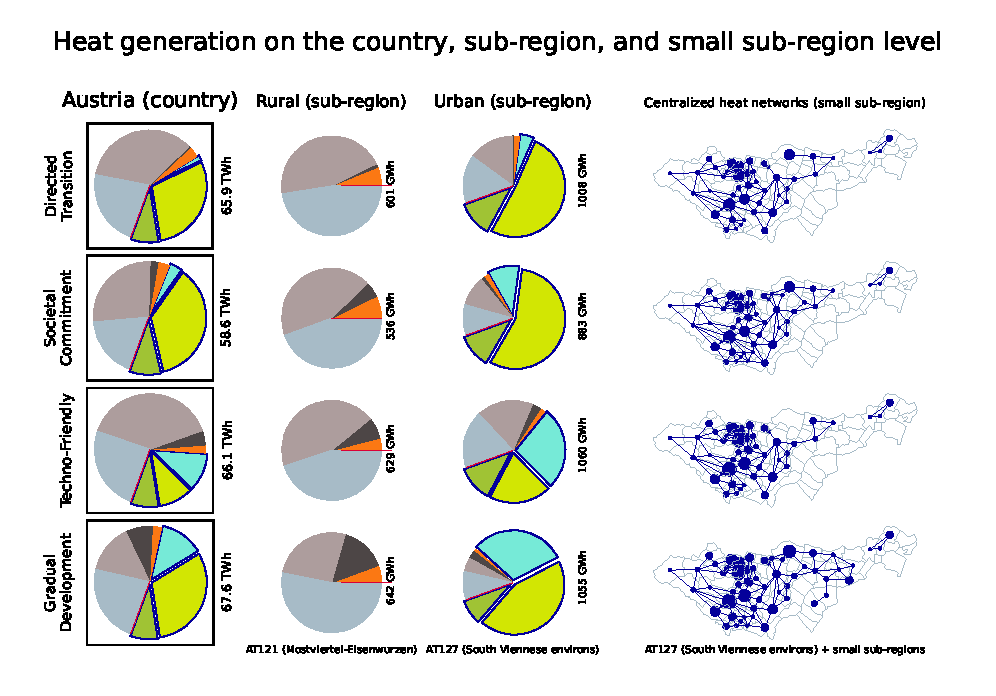
\includegraphics[width=1\linewidth]{figures/4_Results/Spatial_results.eps}
	\caption{Low temperature heat technology generation on different spatial granularity levels for the four different storylines. left: heat technology generation mix on the country level. middle: comparison of technologies supplying the low temperature heat demand in a rural and urban sub-region. right: Centralized heat network topology (size of the points represent the amount of local heat demand supplied by the centralized heat network)}
	\label{fig:res1}
\end{sidewaysfigure}
\newpage
\subsection{Austrian sub-regions with high potentials for centralized low temperature heat supply resulting from aiming the decarbonization}\label{res:3}
%Hier steht etwas.
%% bereits angedeutet, dass es in bestimmten regionen (abbildung 1 urban) technologien wärme versorgen, die netzwerke brauchen
%% diese sind vorwiegend im dichtbesiedelte bzw. urbanen gebiet liegen
%% Abbildung zeigt die österreich karte heat map für beides, network based und on-site. 
%% in dieser arbeit wird wie bereits im wesentlichen recht strikt getrennt zwischen diesen beiden. 

\begin{sidewaysfigure}
	\centering
	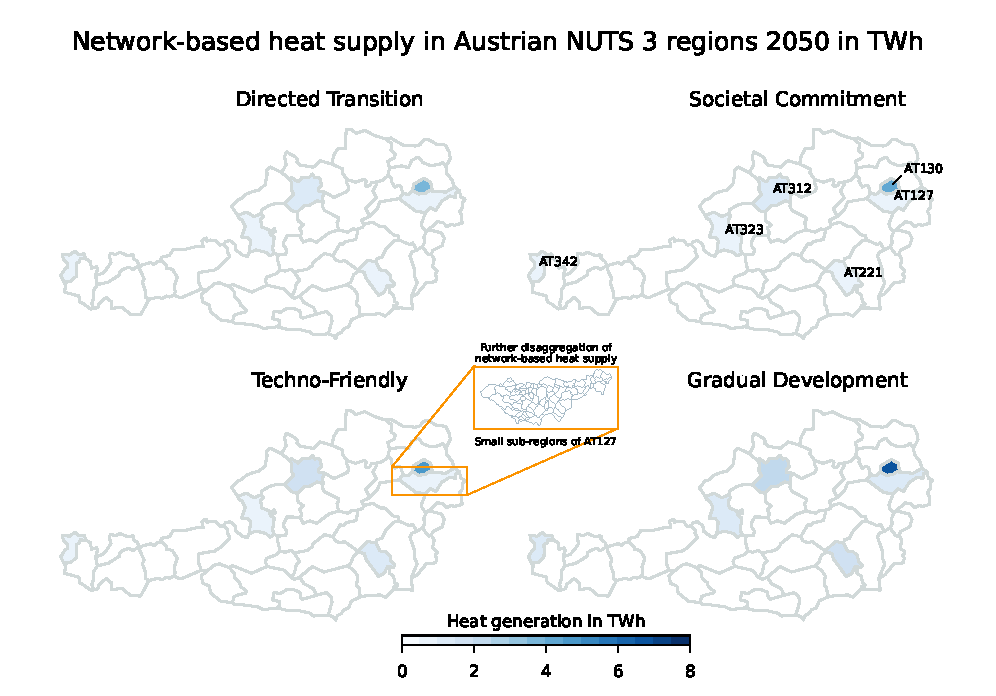
\includegraphics[width=1\linewidth]{figures/4_Results/Heatmap.eps}
	\caption{Low temperature heat technology generation on different spatial granularity levels for the four different storylines. Left: heat technology generation mix on the country level. Middle: comparison of technologies supplying the low temperature heat demand in a rural and urban sub-region. Right: Centralized heat network topology (size of the points represent the amount of local heat demand supplied by the centralized heat network)}
	\label{fig:res2}
\end{sidewaysfigure}

\subsection{Low temperature heat network topology on the small sub-region level}\label{res:4}




\subsection{Comparison of existing and future projections of low temperature heat networks using heat and population density}\label{res:5}




%This section presents and discusses the results of the invesigated Austrian case study. Section \ref{res:1} elaborates on the heat generation technology options supplying the low temperature heat demand on the sub-region level. Section \ref{res:2} deals with the topology of low temperature heat networks on the small sub-region (LAU) level. Finally, Section \ref{res:3} compares the heat densities of low temperature heat networks obtained by downscaling with those from existing networks. 












%Erster Absatz beschreibt die Abbildung mit den Stacked bar plot. Man sieht, dass die network-based technologies nur in den dichtbesiedelten Gebieten genutzt werden. Dort einen erheblichen Anteil ausmachen. Wie viel machen sie dort aus? eventuell ein paar zahlen hier einfügen. unterschiedliche Mengen in den vier szenarien, wo unterscheiden sie sich - in wien ist starker unterschied zu sehen. restliche gebiete mit network-based eher gleichbleibend. wie wird es in den anderen gebieten versorgt. welche dominierenden technologien/energy carriers gibt es dort.
%
%Für weitere Überlegungen ist network-based weiter untersucht. abbildung 3 zeigt die heatmap von centralized heat supply. im folgenden kapitel sind nun die ergebnisse weiter hinuntergebrochen auf LAU ebene um dortige topologien zu untersuchen. 
%
%\begin{sidewaysfigure}
%	\centering
%	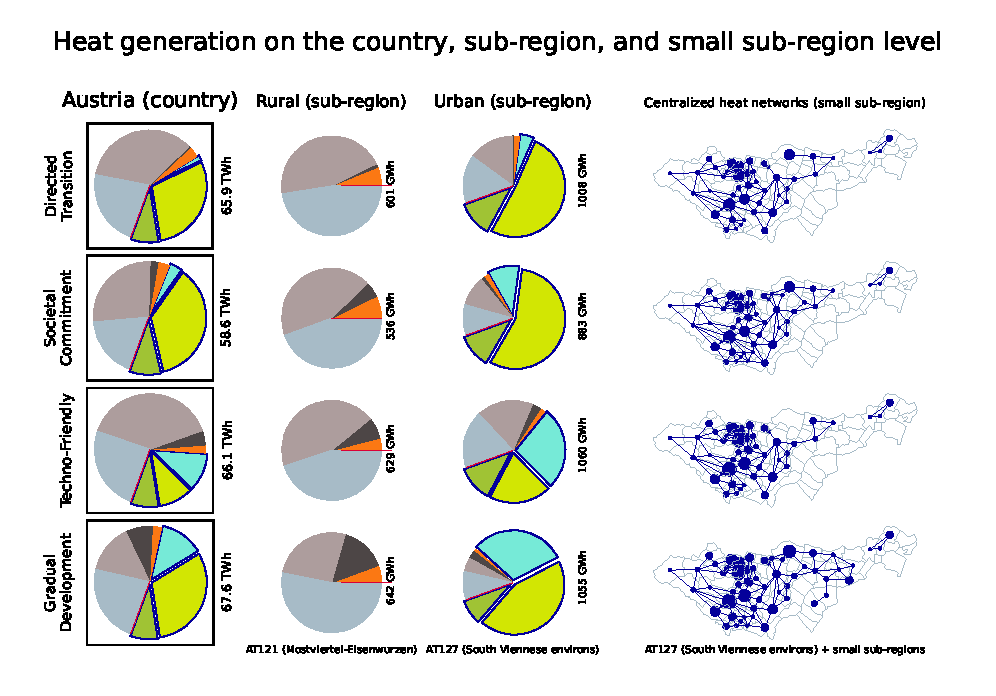
\includegraphics[width=1\linewidth]{figures/4_Results/Spatial_results.eps}
%	\caption{}
%	\label{fig:res1}
%\end{sidewaysfigure}
%
%\begin{sidewaysfigure}
%	\centering
%	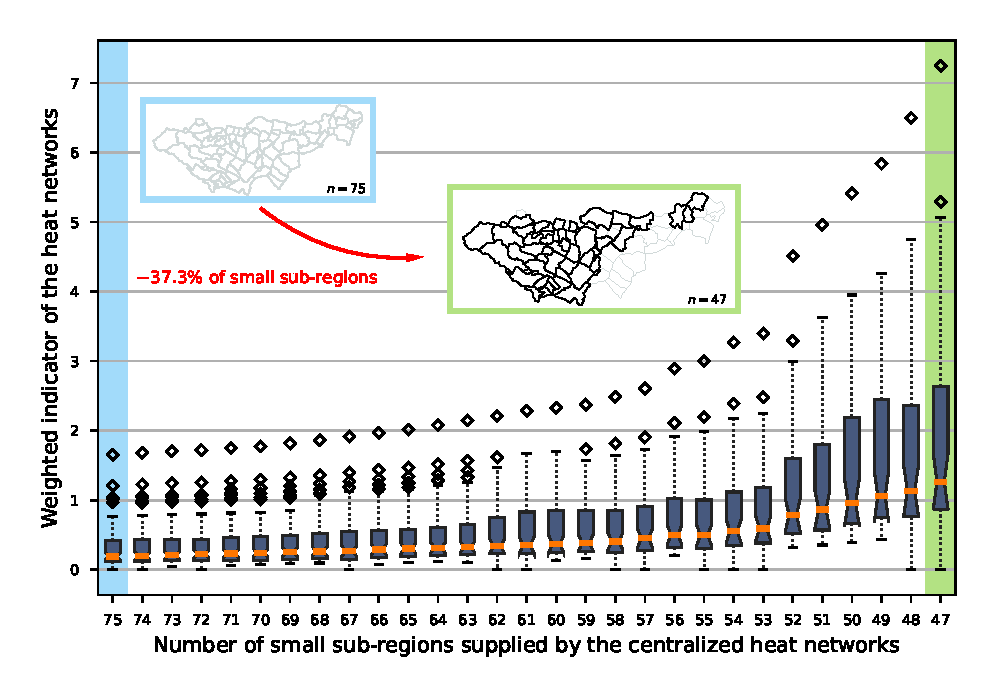
\includegraphics[width=1\linewidth]{figures/4_Results/boxplot.eps}
%	\caption{}
%	\label{fig:res1}
%\end{sidewaysfigure}
%
%\begin{sidewaysfigure}
%	\centering
%	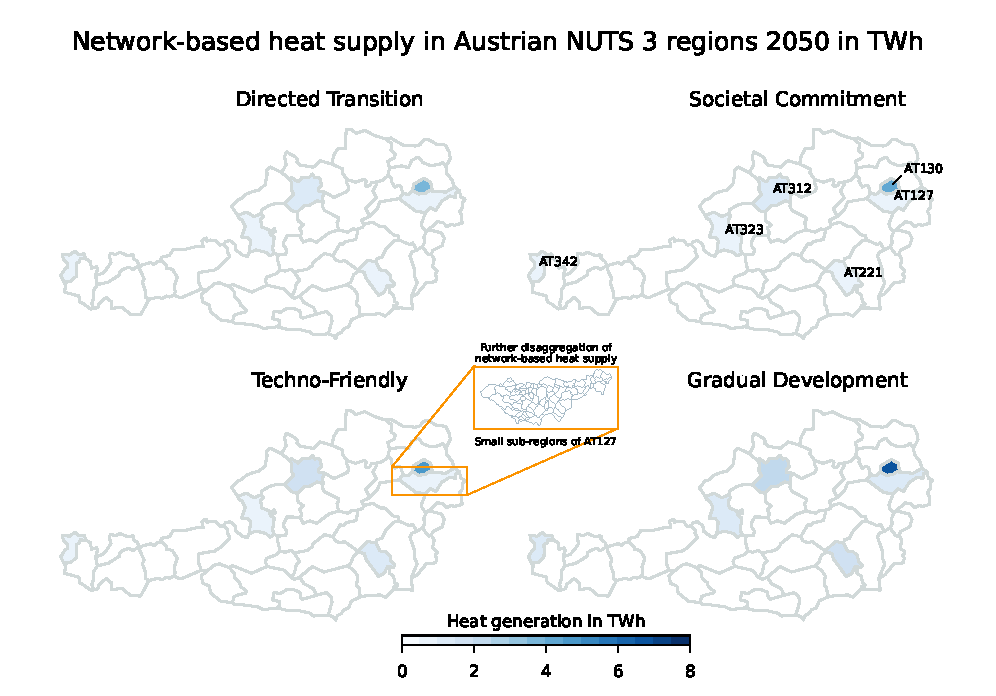
\includegraphics[width=1\linewidth]{figures/4_Results/Heatmap.eps}
%	\caption{}
%	\label{fig:res1}
%\end{sidewaysfigure}
%
%\begin{sidewaysfigure}
%	\centering
%	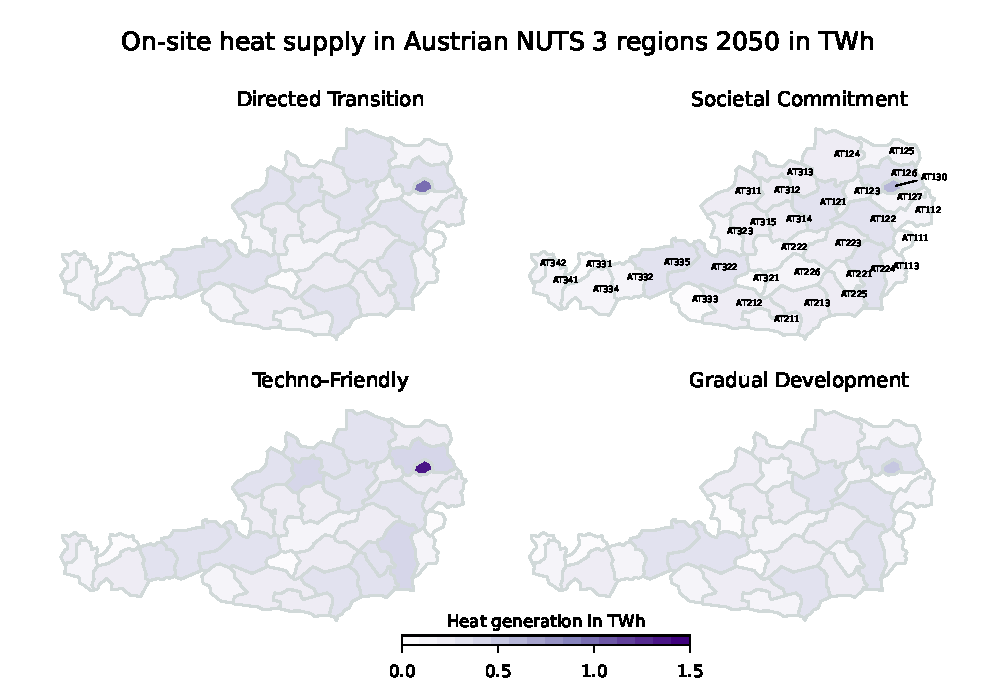
\includegraphics[width=1\linewidth]{figures/4_Results/Heatmap_on-site.eps}
%	\caption{}
%	\label{fig:res1}
%\end{sidewaysfigure}



%\begin{sidewaysfigure}
%	\centering
%	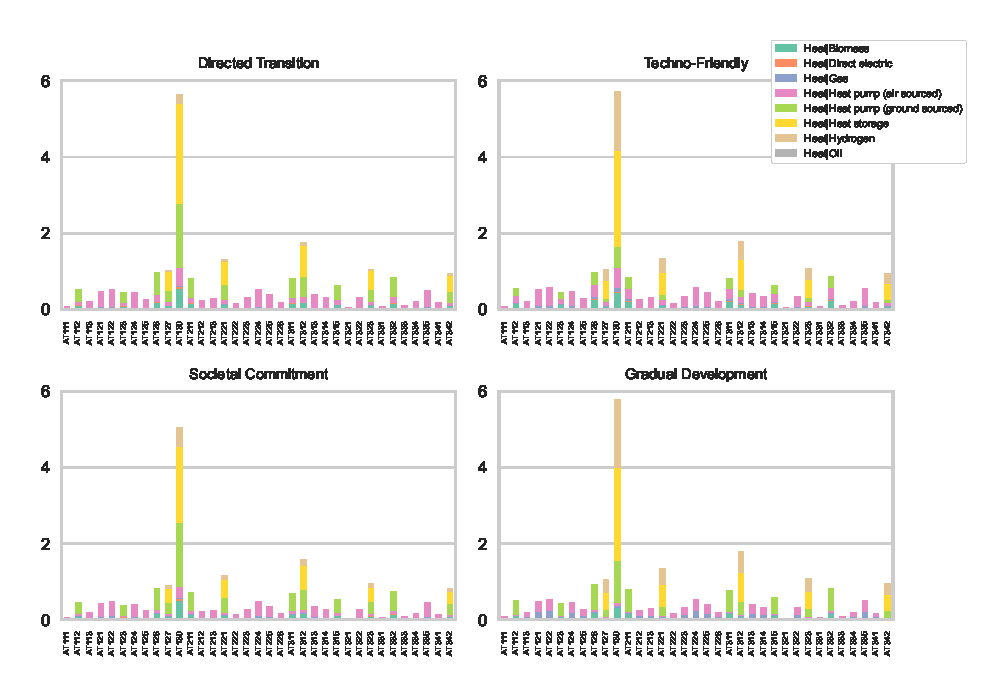
\includegraphics[width=1\linewidth]{figures/4_Results/NUTS3.eps}
%	\caption{}
%	\label{fig:res1}
%\end{sidewaysfigure}
%
%\begin{sidewaysfigure}
%	\centering
%	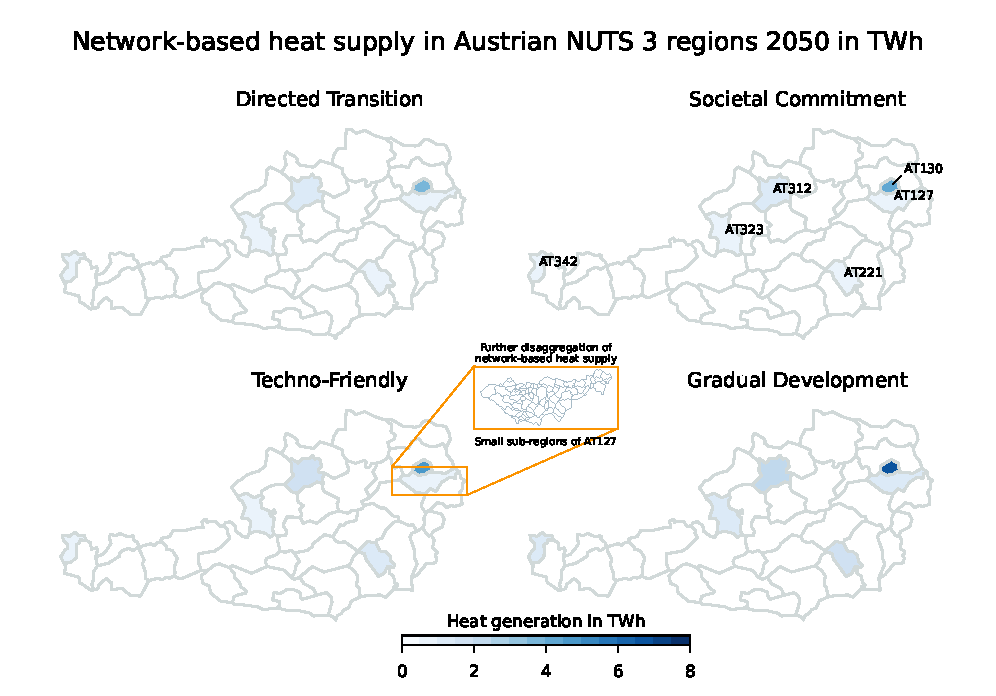
\includegraphics[width=1\linewidth]{figures/4_Results/Heatmap.eps}
%	\caption{}
%	\label{fig:res2}
%\end{sidewaysfigure}

%\newpage
%\subsection{Centralized heat supply topology on the small sub-region (LAU) level}\label{res:2}
%Die untersuchung ist für alle NUTS 3 regions durchgeführt, die centralized heat supply haben. im nachfolgenden werden die ergebnisse von 1 oder 2 sub-regions detailliert dargestellt. In der Comparison sind dann die ergebnisse von allen regionen berücksichtigt. für weitere ergebnisse, deren darstellung bzw. genauen zahlenwerten wird auf das entprechende open-source repository auf github verwiesen, dass alles beinhaltet. 
%
%Dann hier eine abbildung von linear downscaling auf LAU ebene und wie die Topology aussehen würde (anmerkung, dass dies vor anwendung von algorithmus 2 der fall wäre). Dem gegenüber ist die nächste abbildung dann das ergebnisse für dieses gebiet nach algorithmus 2. wie verändert sich das netzwerk, welche punkte sind verloren gegangen und welche haben an menge hinzubekommen. bedeutet also, dass on-site generation lokal ersetz wurde und nun bevorzugt über das netzwerk versorgt wird wohingegen der entgegengesetzte prozess bei anderen knoten zu erkennen ist. 
%
%\subsection{Comparison of the results with existing heat network infrastructures}\label{res:3}
%Vergleich wird über die heat densities angestellt. 



